\documentclass[a4paper,dvipdfm]{article}
\usepackage[margin=1in]{geometry}
\usepackage[utf8]{inputenc}
\usepackage[brazil]{babel}
\usepackage{indentfirst}
\usepackage{cite}
\usepackage{url}
\usepackage{graphics}
\usepackage{graphicx}
\usepackage{caption}
\usepackage{subcaption}
\usepackage[acronym]{glossaries}
	

\title{Como o spam afeta a comodidade do Correio Eletrônico}
\author{Bianca Madoka Shimizu Oe\\
		Gustavo Shinji Inoue\\
		Rafael Umino Nakanishi}

\makeglossaries

\newacronym{acm}{ACM}{Association for Computing Machinery}
\newglossaryentry{email} {
	name={e-mail}, 
	description={Correio eletrônico, termo usualmente utilizado para denotar a mensagem eviada por este meio}
}
\newglossaryentry{cabecalho} {
	name={cabeçalho}, 
	description={Parte do e-mail que contem informações suplementares de transmissão. Entre seus campos, são encontrados endereço do emissor, endereço do receptor, endereço de resposta, data de emissão, tipo do conteúdo e assunto}
}
\newglossaryentry{falsopos} {
	name={falso-positivo}, 
	description={Classificação errônea na qual, para este contexto, um e-mail legítimo é classificado como spam}
}
\newglossaryentry{captcha} {
	name={CAPTCHA}, description={\emph{Completely Automated Public Turing test to tell Computers and Humans Apart}. Teste criado para diferenciar seres humanos de máquinas. Consiste em imagens de mensagens distorcidas para evitar a interpretação automática por máquinas}
}
\newglossaryentry{spambot} {
	name={spambot},
	description={Bot projetado para enviar spam de forma massiva, automaticamente}
}
\newglossaryentry{bot} {
	name={bot}, 
	description={Softwares criados para realizar alguma tarefa de forma automatizada}
}
\newglossaryentry{cadmarkov} {
	name={Cadeia de Markov},
	description={Conjunto de estados no qual um processo ocorre. O processo inicia em um estado e se move sucessivamente, transicionando entre estados, a cada passo. O estado para o qual o processo se move depende unicamente, de forma probabilística, do estado em que ele se encontra atualmente},
	plural={Cadeias de Markov}
	
}
\newglossaryentry{crm114} {
	name={\emph{CRM114}, 
	description={Software anti-spam baseado em técnicas estatísticas para a filtragem e classificação de dados. Seu código fonte na linguagem C é disponibilizado sob a licença \emph{GPL}}}
}
\newglossaryentry{gpl} {
	name={\emph{GPL}, 
	description={\emph{General Public License}. Licença para software livre}}
}
\newglossaryentry{whitelist} {
	name={whitelist}, 
	description={Lista de endereços de e-mail de remetentes legítimos, previamente validados}
}
\newglossaryentry{blacklist} {
	name={blacklist}, 
	description={Lista de mensagens classificadas como spam}
}
\newglossaryentry{mta} {
	name={MTA},
	description={Mail Transfer Agent. Software que transfere mensagens de correio eletrônico de um cliente para outro, baseado em uma arquitetura cliente-servidor}
}
\newglossaryentry{threshold} {
	name={threshold}, 
	description={Valor utilizado como limitante para uma classificação}
}

\begin{document}
\maketitle
%\newpage

\begin{abstract}
	O uso do correio eletrônico se tornou uma necessidade pessoal com o advento da tecnologia. Com esse novo meio de comunicação há maior praticidade e agilidade na troca de mensagens, de forma que não é necessário se locomover longas distâncias para conversar com outras pessoas.

	Entretanto, a facilidade adquirida também permite o envio de milhares de mensagens eletrônicas em poucos segundos, que podem ser mensagens importantes, como um aviso de uma empresa de grande porte para seus funcionários, ou \emph{spam}, um fenômeno que cresce dia após dia.

	((Mudar isso))
	Nosso objetivo, nesta monografia, é mostrar como o spam vem trazendo inconveniências os usuários de \gls{email}.
	Mostraremos a origem da palavra e seus usos nos dias atuais. 
	((colocar algo como em seguida aqui)) métodos utilizados para separar mensagens importantes de spam.
	Em seguida, alguns exemplos de como esse tipo de mensagem traz desconforto para quem o recebe. 
	Por fim, um estudo de caso, analisando as violações dos códigos da \gls{acm}~\cite{ACM} e a conclusão.
\end{abstract}

\newpage

\tableofcontents
\newpage


\section{Introdução}
	Nesta seção será feita uma breve descrição de como o termo spam (para falar de mensagens indesejadas) foi originado, seguida de ((blablabla)).

	\subsection{Origem do termo}
		A aparição da palavra Spam que originou sua utilização atual ocorreu no episódio 12 da segunda temporada de uma série britânica de comédia chamada \emph{Monty Python's Flying Circus}. 
		Spam é uma mistura de carnes de porco apimentadas e enlatadas, vindo de \emph{SPiced hAM} (Figura \ref{fig:spam}), criado pela empresa estadunidense \emph{Hormel Foods Corporation}.

		Durante o episódio, personagens discutem sobre o cardápio de um café. 
		A carne enlatada é um ingrediente presente em todos os pratos do estabelecimento, sendo considerada algo indesejável por um dos personagens, e, durante a discussão, "Spam" foi dito mais de 50 vezes em menos de 4 minutos.

		Apesar de não se saber ao certo quando o termo começou a ser utilizado para denotar mensagens indesejadas, atualmente ele é vastamente utilizado, principalmente para  se referir a e-mails de propagandas inconvenientes.
		
		\begin{figure}[ht]
			\centering
			
\includegraphics [height=5cm]{Imagens/spam/spam.png}
			\caption{Lata de presunto apimentado enlatado}
			\label{fig:spam}
		\end{figure}

	\subsection{Spam ((na atualidade))}
		A empresa especializada em segurança \emph{M86 Security Labs}~\cite{m86} separa spam em 13 categorias listadas abaixo:
		\begin{description}
			\item [Fraude] Seu objetivo é fazer o destinatário acreditar que ganhou algo, como um prêmio.
			\item [Adulto] Possui conteúdo pornográfico e oferece cadastro gratuito a \emph{sites} adultos ou a serviços de acompanhantes.
			\item [Financeiro] É relacionado a financiamentos e oferecimento de crédito falso.
			\item [Ações] Anuncia ações de empresas para causar o aumento do preço das mesmas.
			\item [Farmacêuticas] Informa sobre vários tipos de drogas e remédios, geralmente promete uma pele melhor, mais energia, perda de peso, entre outros. 
			Como um exemplo, tem-se o Viagra.
			\item [Phishing] Tenta imitar e-mails legítimos enviados por empresas para conseguir dados e/ou credenciais de seus clientes.
			Seus alvos mais populares são bancos, \emph{eBay} e \emph{PayPal}.
			\item [Diplomas] Anuncia qualificações como diplomas de universidades ou cursos de treinamento.
			\item [Réplicas] Anuncia imitações baratas de produtos como bolsas, relógios e celulares.
			\item [Software] Anuncia softwares baratos, usualmente prometendo venda de softwares \gls{oem}.
			\item [Malware] Contem anexos maliciosos ou \emph{links} que levam a \emph{websites} com vírus.
			\item [Jogos de azar] Promove cassinos ou \emph{sites} de pôquer, que geralmente oferecem bônus por cadastramento.
			\item [Relacionamento] Podem ser incluídos na categoria de fraudes, em que mulheres ou homens que fingem ser mulher tentam criar um relacionamento para extorquir dinheiro.
			\item [Outros] Não são classificados nas categorias supracitadas.
		\end{itemize}

		Dentro dessas classes, 

		Segundo , $72.7\%$ dos e-mails recebidos são spam e $56\%$ dessas mensagens são farmacêuticas.
		A distribuição de emissores de spam pelo mundo pode ser vista na Figura \ref{fig:spamworld}.

	\begin{figure}[ht]
		\begin{subfigure}[b]{\textwidth}
			\centering
			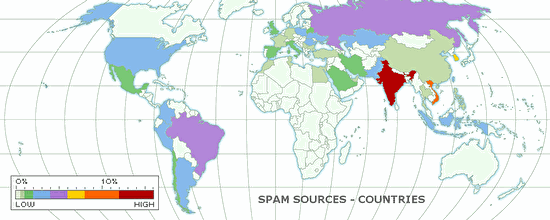
\includegraphics[height=5cm]{Imagens/m86security/spam-country-map.png}
			\caption{Mapa de emissores de spam((mude isso))}
		\end{subfigure}
		~
		\begin{subfigure}[b]{0.47\textwidth}
			\centering
			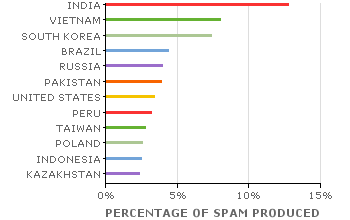
\includegraphics[height=5cm]{Imagens/m86security/spam-country-bar.png}
			\caption{12 países que mais emitem spam}
		\end{subfigure}
		~
		\begin{subfigure}[b]{0.47\textwidth}
			\centering
			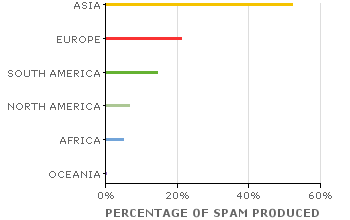
\includegraphics[height=5cm]{Imagens/m86security/spam-continent-bar.png}
			\caption{Percentual de spam emitido por continente}
		\end{subfigure}
		\caption{Emissão de spam no mundo}
		\label{fig:spamworld}
	\end{figure}

\section{Filtros de Spam}
	Para acompanhar o aumento do número e da variedade de spams, vem sendo criados vários métodos para separar mensagens importantes de propagandas.
	São inúmeras as abordagens utilizadas. 
	Algumas se baseiam no \gls{cabecalho} da mensagem, outras na frequência das palavras utilizadas.
	Nas seções seguintes, serão brevemente discutidas algumas estratégias utilizadas no combate ao spam, e, como um exemplo, serão mostrados alguns dos filtros utilizados pelo \emph{Gmail}((citar?)).

	\subsection{Filtro baseado na estrutura do texto}
		Este tipo de filtro se baseia em cadeias específicas do cabeçalho do e-mail, como, por exemplo, a língua na qual foi escrito e o tipo do conteúdo da mensagem.

		Estes filtros podem ser facilmente criados pelos próprios usuários em grandes servidores de e-mail, e tem como objetivo não só detectar spam, mas também separar mensagens relevantes em categorias.

		A vantagem desta estratégia é o alto nível de personalização permitido, já que cada usuário pode criar seu próprio filtro dependendo do tipo de spam recebido. 
		Além disso, a probabilidade de haver falsos-positivos é menor, já que é o próprio usuário que escolhe os parâmetros de filtragem.
		
		Sua desvantagem é a possível necessidade de criação de vários filtros para se obter uma separação eficaz.


	\subsection{\emph{Whitelist}/Verificação}
		Uma abordagem mais agressiva para a filtragem de spam é a utilização de \emph{Whitelist} em conjunto com a verificação automática.

		Qualquer endereço que esteja nesta \emph{whitelist} tem sua mensagem enviada sem maiores problemas.
		Caso o endereço não esteja contido na lista, o \emph{\gls{mta}} envia uma mensagem de volta para o remetente, com instruções que, ao serem seguidas, adicionam o endereço do remetente na \emph{whitelist}.

		Como a maioria das mensagens de spam possui endereços de resposta falsos, as instruções não seriam seguidas e o e-mail não chegaria à caixa de entrada do destinatário.
		Caso o \emph{spammer} decida fazer o que lhe foi dito, ele será adicionado à lista, porém isso o torna mais facilmente rastreável.
		
		Apesar de ser uma maneira eficaz de diminuir os spams, ela pode prejudicar usuários legítimos que não podem ou querem atender a essa exigência, já que isso implicaria no não recebimento de sua mensagem.

		Como um exemplo deste tipo de abordagem, tem-se o \emph{Corlive.com}~\cite{corlive}, que é um servidor de e-mail que utiliza \emph{Captcha}~\cite{captcha} para validar os e-mails enviados e não permitir que \emph{bots} enviem spam.

	\subsection{Distribuição adaptativa de \emph{blacklist}}
		A \emph{blacklist} é formada por mensagens que foram classificadas como spam por usuários ou mesmo por endereços especiamente criados por servidores para atrair spam.

		Ao receber uma mensagem, o MTA utiliza um filtro por \emph{blacklist} para determinar se mesma é um spam conhecido, e ela só é enviada à caixa de entrada do destinatário caso ela não seja classificada como ilegítima.

		Esta estratégia se baseia no uso de técnicas estatísticas para sumarizar o conteúdo de um mensagem de forma que pequenas mutações no spam não impeçam seu reconhecimento.

		A probabilidade de haver falsos-positivos é pequena, já que é necessária uma marcação na mensagem para que ela entre na \emph{blacklist}. Além disso, quando ocorre uma marcação errônea de mensagens vastamente enviadas, como informativos, o gerenciador da lista pode desmarcá-las.
		
		Como é necessária a verificação da mensagem em um servidor, a performance deste método comparada a outros é baixa, sendo ele bastante lento.

		Um exemplo de software que implementa esta abordagem é o \emph{Pyzor}~\cite{pyzor}, um software implementado em \emph{Python} sob a licença \emph{GPL}.

	\subsection{Ranking baseado em regras}
		Este filtro possui regras de ranking, principalmente expressões regulares, e tenta fazer correspondências entre o padrão e a mensagem. 
		Cada equivalência adiciona ou diminui pontos da mensagem.
		
		Se a quantidade de pontos do e-mail exceder um determinado threshold, é classificado como spam, caso contrário, é classificado como uma mensagem legítima.

		A dificuldade deste tipo de filtro é que, apesar de existirem regras que são contantes com o decorrer do tempo, como endereço de resposta falso ou áudio como tipo de conteúdo, há outras que mudam com o tempo, como os produtos dos quais os spams fazem propaganda, e isso causa a necessidade constante de atualização das regras.

		Um software que implementa este tipo de filtro é o \emph{SpamAssassin}~\cite{spamassassin}, um projeto open-source da \emph{Apache}.

	\subsection{Filtro Bayesiano}
		A abordagem do filtro Bayesiano, criado por Paul Graham, é a utilização de modelos Bayesianos de probabilidade para determinar se uma mensagem é legítima ou não.

		É criado um dicionário de palavras contendo a probabilidade de ela estar em um spam e a probabilidade de estar em uma mensagem válida. Esse dicionário é utilizado para calcular a probabilidade geral de a mensagem ser um spam, com base na teoria da probabilidade condicional de Bayes.

		Este filtro possui traz vários benefícios como ser automatizável, ou seja, não são necessárias pessoas para definir os valores de probabilidade, já que ele pode aprender, isto é, adicionar novas palavras ou modificar a probabilidade de uma palavra de acordo com a marcação de um e-mail como spam ou válido.

		Além disso, sua implementação e a teoria em que se baseia são extremamente simples e sua performance é melhor que a de filtros baseados em regras.
		
		Um software que implementa o filtro Bayesiano é o \emph{SpamBayes}~\cite{spambayes}, disponível para os serviços de e-mail \emph{Gmail}, \emph{MSN Hotmail}, \emph{Yahoo! Mail}, entre outros.

	\subsection{Filtro Markoviano}
		O filtro Markoviano é um filtro estatístico baseado na teoria de Cadeias de Markov~\cite{markov}, na qual o próximo estado depende unicamente do estado atual, e leva em consideração a probabilidade de transição entre uma palavra e outra, ou seja, dada uma palavra, ele tenta predizer qual é a próxima.

		Diferentemente do filtro Bayesiano, que é baseado em palavras independentes, o filtro Markoviano trabalha em cima de frases, e por isso, seu desempenho tende a ser maior, já que utiliza uma abordagem holística do texto.
		
	Esta estratégia é utilizada no filtro de spam \emph{CRM114}, juntamente com outras abordagens que não serão discutidas neste trabalho. Seu desempenho foi testado para diferenciar documentos japoneses confidenciais de não confidenciais, e a acurácia obtida foi maior que $99\%$ e taxa de falsos-positivos foi menor que $5.3\%$~\cite{fmarkov:japtest}.

	\subsection{Gmail}
		A técnica mais utilizada pelo provedor de serviços \emph{Gmail} é o aprendizado baseado em instâncias, chamado pelo provedor de \emph{Community clicks}, ou seja, a cada mensagem que o usuário marca como spam ou como mensagem legítima, seus filtros são aprimorados.

		Outra técnica é o aprendizado de máquina usado para combinar e indexar os conjuntos de busca do buscador Google, que permite a junção de vários fatores para identificar mensagens semelhantes e classificá-las como spam.
		Além disso, são aplicadas ferramentas como \emph{OCR} de outro serviço da empresa, o \emph{Google Book Search}, serviço de busca em livros (podem ser imagens), para identificar spams em forma de imagens.

		A filtragem também é feita por endereço, ou seja, se um usuário marca a mensagem de um emissor como spam várias vezes, próximas mensagens enviadas por esse endereço irão para a caixa de spam automaticamente, como um filtro por distribuição de blacklist.

		A eficácia do filtro pode ser vista na Figura \ref{gmail:chart}.

		\begin{figure*}[ht]
			\centering
			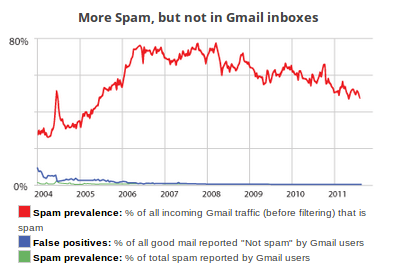
\includegraphics[height=7cm]{Imagens/gmail/spamchart.png}
			\caption{Percentual de filtragem ao longo dos anos}
			\label{gmail:chart}
		\end{figure*}
		

\section{Casos Reais}

\section{Estudo de Caso}
\subsection{((História))}
\subsection{Potenciais benefícios e vulnerabilidades}
\subsection{Decisão consensual}

\section{Conclusão}

\newpage
\printglossaries
\addcontentsline{toc}{section}{Glossário}

\newpage
\bibliography{refs}
\bibliographystyle{acm}
\addcontentsline{toc}{section}{Referências}

%\newacronym{acm}{ACM}{Association for Computing Machinery}
\newglossaryentry{email} {
	name={E-mail}, 
	description={Correio eletrônico, termo usualmente utilizado para denotar a mensagem eviada por este meio.}
}
\newglossaryentry{cabecalho} {
	name={cabeçalho}, 
	description={Parte do e-mail que contem informações suplementares de transmissão. Entre seus campos, são encontrados endereço do emissor, endereço do receptor, endereço de resposta, data de emissão, tipo do conteúdo e assunto.}
}
\newglossaryentry{falsopos} {
	name={falso-positivo}, 
	description={Classificação errônea na qual, para este contexto, um e-mail legítimo é classificado como spam}
}
\newglossaryentry{captcha} {
	name={CAPTCHA}, description={\emph{Completely Automated Public Turing test to tell Computers and Humans Apart}. Teste criado para diferenciar seres humanos de máquinas. Consiste em imagens de mensagens distorcidas para evitar a interpretação automática por máquinas.}
}
\newglossaryentry{spambot} {
	name={spambot},
	description={Bot projetado para enviar spam de forma massiva, automaticamente.}
}
\newglossaryentry{bot} {
	name={bot}, 
	description={Softwares criados para realizar alguma tarefa de forma automatizada.}
}
\newglossaryentry{cadmarkov} {
	name={Cadeia de Markov}, description={Conjunto de estados no qual um processo ocorre. O processo inicia em um estado e se move sucessivamente, transicionando entre estados, a cada passo. O estado para o qual o processo se move depende unicamente, de forma probabilística, do estado em que ele se encontra atualmente.}
}
\newglossaryentry{crm114} {
	name={\emph{CRM114}, 
	description={Software anti-spam baseado em técnicas estatísticas para a filtragem e classificação de dados. Seu código fonte na linguagem C é disponibilizado sob a licença \emph{GPL}}}
}
\newglossaryentry{gpl} {
	name={\emph{GPL}, 
	description={\emph{General Public License}. Licença para software livre.}}
}
\newglossaryentry{whitelist} {
	name={whitelist}, 
	description={Lista de endereços de e-mail de remetentes legítimos, previamente validados.}
	}
\newglossaryentry{blacklist} {
	name={blacklist}, 
	description={Lista de mensagens classificadas como spam.}
	}
\newacronym{mta}{MTA}{Mail Transfer Agent}{
	description={Software que transfere mensagens de correio eletrônico de um cliente para outro, baseado em uma arquitetura cliente-servidor.}
}
\newglossaryentry{threshold} {
	name={threshold}, 
	description={Valor utilizado como limitante para uma classificação.}
}


\end{document}
